\subsection{Registration}
Visitors can register to PowEnJoy through mobile application. This operation requires the visitor to fill a registration form with personal data and accept PowEnJoy terms and conditions, including personal data policies, according to local law. The system requires the visitor personal information as name, surname, and birthday, payment information ( as a credit card or a paypal account) and proof of the possesion of a valid driver license
If any of the previous requirements are not met or any input is invalid, the registration fails and the system asks the visitor to repeat the process. Other- wise, a verification email containing the password of the account is sent to the provided email address. To validate his account the visitor needs to login one time with the provided password.
\paragraph{Scenario}
Meg is a student. She has heard about PowEnJoy and, finding it an easy and ethical way to travel, wants to subscribe to it.
Therefore, she download the mobile application from the store and clicks on Register in the main screen. She fulfil the form, accepts the term and conditions  and she click Confirm. However, the system cannot verify Meg's driver license because she forgot to put the photo that prove the possession of it. It therefore asks Meg to take the picture from her mobile's camera. Once she has enter everything correctly she click on Confirm, this time the application valid his credential and tell to meg to check her emails, she will find the confirmation of the correct registration and the given by the software. Meg read her emails and can finally open the application again and login with the given password and the email she gave before.
\paragraph{Diagrams}
\begin{figure}[H]
   \begin{center}
    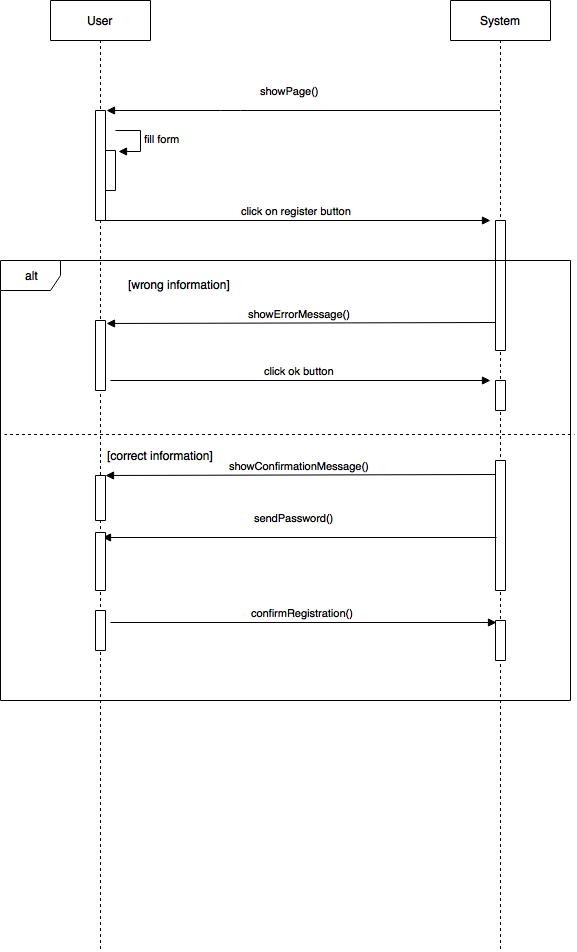
\includegraphics[width=\textwidth]{Resources/registerSequence.png}
    \caption{Registration sequence}
   \end{center}
    \label{fig:regSequence}
\end{figure}
\paragraph{Special Requirements}
\begin{itemize}
	\item Visitor can abort the registration process at any time.
	\item The password in the email must be used within 1 day, otherwise the registration is deleted along with the visitor?s info.
	\item Registration form contain the following information (fields):
	\begin{itemize}
		\item Email address.
		\item First name.
		\item Surname.
		\item Address.
		\item City.
		\item Postal Code.
		\item Credit card code.
		\item Expiration date of the credit card.
		\item Secure code of the credit card.
		\item Driver license code.
		\item Expiration of driver license.
		\item Photo of a driver license.
	\end{itemize}
	\item Email address cannot be the same as ones from other PowerEnJoy users.
	\item The photo of the driver license must be taken by the camera of the mobile.
\end{itemize}

\subsection{Login}
Visitors on PowerEnJoy mobile application may access to an existing registered user account providing its corresponding email address and password. In case the submitted info do not match with any existing account info, the system notifies the visitor that the email address doesn?t exist, or that it exists, but the submitted password is wrong. In case a user forgets his/her password, the system allows him/her to retrieve it, automatically creating a new password, setting it as the user?s one and sending it to the provided email address.
\paragraph{Scenario}
\begin {enumerate}
\item Freddy is user of PowerEnJoy. He already downloaded the application from the store and he has already done the registration from the application. He cannot remember the password given from the system during the registration time. Therefore he open the app on the home page and he is redirect to the login page. He click then on the forget password link and the application ask him his email address. He insert the email address and then the application show another message telling the user to check the emails. Once he has received the new password, Freddy can finally open again the application and login with the his email address and the new password.
\item Eleonor is a lawyer familiar with the PowerEnJoy system, she have recently changed phone and she has already download the application again. She open the application and she is redirect in the login page. she fills both fields and clicks on ?Log in?. The system verifies her info: the operation ends successfully, and she gains access to the user homepage.
\end{enumerate}
\paragraph{Diagrams}
%%here
\paragraph{Special Requirements}
\begin{itemize}
	\item Visitors must fill the "email field" with an existing email address in order to successfully log in.
	\item Visitors must fill the ?password? field with the only password correspond- ing to the submitted email address in order to successfully log in.
	\item The system will ignore log in requests if at least one of the ?email? and ?password? fields are left blank.
	\item The system allows visitors to retrieve their password if they forget it, by clicking ?Forgot password??.
	\item The system requires visitors to submit an existing email address in order to retrieve their password.
	\item The system will take care of assigning the user a new password, when he/she states to have lost the previous one.
	\item The system will take care of sending to the email address submitted by the visitor the new assigned password, when he/she states to have lost the previous one.
	\item The system allows visitors to retrieve their password once a day.
	\item The system remember the user's credential until the user decide to logout.
\end{itemize}

\subsection{Reserve car}
Logged user on PowerEnJoy can look for cars near his/her position, or next to a specify address, and reserve one for a rent. This operation is possible using the map on the home page of the application that indicate with a marker the position of the car, only the cars that are in a free state can be reserved and are visible on the map
\paragraph{Scenario}
Francis needs to go home from a dinner with his friends. It is late and there are public transport anymore. He is already registered and successfully logged-in in the PowerEnJoy application. He decided to reserve a car using the application. He opens the application and he is directly redirect to the application home page that contains the map with the markers of cars near him. He choose a marker and he click on it. The app show him the information of the car as its battery charge and its position. The car is really close to him therefore he click on the button reserve and he moves next to the car. Meanwhile the application shows him the  a timer, the vehicle registration plate, his position and the position of the car. Once the Francis arrives next to the car the app shows him a button to open the car. The rent start when Francis start the engine of the car.
%Another scenario with a men who can't reach the car until in one hours?
\paragraph{Diagrams}
\begin{figure}[H]
   \begin{center}
    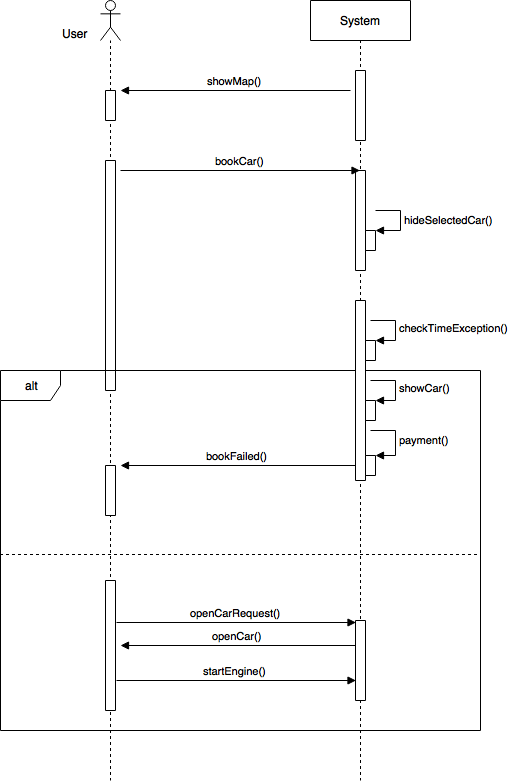
\includegraphics[width=\textwidth]{Resources/bookSequenceDiagram.png}
    \caption{Registration sequence}
   \end{center}
    \label{fig:bookCarSequence}
\end{figure}
\paragraph{Special Requirements}
\begin{itemize}
	\item A car change is state from \emph{"Reserved"} to \emph{"In use"} only when the engine starts
	\item A car can be reserved and showed on the map only if its state is \emph{"Free"}
	\item A car stays in the \emph{"Reserved"} state for at maximum one hour, if it's not picked-up it return to the state \emph{"Free"}
	\item Each car have a precise position
	\item An user can open the car through the app only if it is near to it
	\item Each user can reserve only one car at the same time
	\item A car can be reserved from only one user at the same time
\end{itemize}

\subsection{End a rent}
Once the user has finish his/her ride he/she have to parks the car in a safe area or a parking, stop the engine and get off the vehicle. The system check if all the requirements to end the rent are respected and close the car. The system wait 5 minute to let the user plug the car if he/she wants to. After the wait time the system send the payment request to the external payment system. The end of a rent can also provide some discount on the final payment or the add some overtaxes.
\paragraph{Scenario}
\begin{enumerate}
	\item Isa is an habitual user of PowerEnJoy. She picked-up a car to cross the city and be ecologic with the system. She has finished her ride and she wants to end the rent. She parks the car near a safe area near her destination and she stops the engine of the car. The safe area, as defined, has a plug to recharge the car so Isa plugs the car just after she has stopped the car. The system notify Isa of the correct end of her rent and show her the final bill, that contain a discount of 30\%, with a message on the application.
	\item Laura took a car of PowerEnJoy to get home with her family, her husband and her tow child. She park the car in a parking but unfortunately the battery of the car is at 10\% and there are no safe area next to Laura's house, the most near is 3.2 Km away. Laura end her rent stopping the engine of the car and receive a message from the app that show her an overtaxes of 30\% due to the position of the parking and the state of the battery life of the car.
	\item Mary rented a car to go home from her university, once she arrives next to her destination she park the car into a parking, she stop the engine and get off the car. Unfortunately the chosen area is not an allowed parking area and the system does not let the her close the car even if nobody is into it. Therefore she moves the car into another parking area and this time, once she followed the procedure, the system close the vehicle and wait 5 minute before charging Mary for her rent. Once the payment is successfully ended the system send a notification to Mary with the resuming of her rent and the bill.
\end{enumerate}
\paragraph{Diagrams}\
\begin{figure}[H]
   \begin{center}
    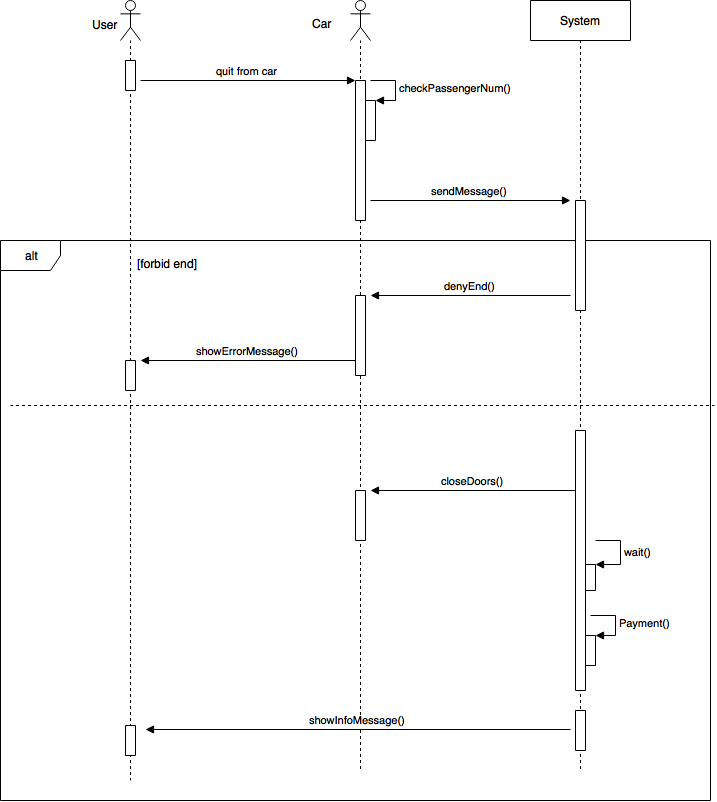
\includegraphics[width=\textwidth]{Resources/endRent.png}
    \caption{Registration sequence}
   \end{center}
    \label{fig:endSequence}
\end{figure}
\begin{figure}[H]
   \begin{center}
    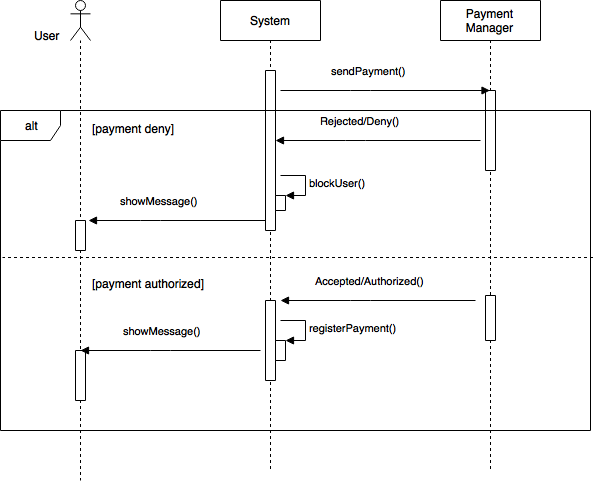
\includegraphics[width=\textwidth]{Resources/Payment.png}
    \caption{Registration sequence}
   \end{center}
    \label{fig:paymentSequence}
\end{figure}
\paragraph{Special Requirements}
\begin{itemize}
	\item If the system detects the user took at least two other passengers into the car, the system applies a discount of 10\% on the last ride.
	\item If a car is left with no more than 50\% of the battery empty, the system applies a discount of 20\% on the last ride.
	\item If a car is left at special parking areas where they can be recharged and the user takes care of plugging the car into the power grid, the system applies a discount of 30\% on the last ride.
	\item If a car is left at more than 3 KM from the nearest power grid station or with more than 80\% of the battery empty, the system charges 30\% more on the last ride to compensate for the cost required to re-charge the car on-site.
	\item The user has five minutes to plug the car if he/she wants a discount
	\item The rent end-up only if the car is closed, parked in a parking/safe area and there is anybody in the vehicle.
	\item The car can be closed only if it is turned off, there is no one in it and if it is parked into a safe/parking area
	\item The discount can be apply only if there are not any overtaxes
	\item Only one discount can be apply to the rent, the one who is the most convenient for the user.
	\item The user has 2 minute before the check of the requirements condition 
\end{itemize}

\subsection{Report problems}
Every logged-in user can report a problem to the PowerEnJoy team during the all time of use of the system. In particular the user has a button to immediately contact the customer service during:
\begin{itemize}
	\item The reservation of a car, in case the car is not opened by the system.
	\item The rent of a car, in case of accident or problem due to the system.
	\item The charge of a car, in case some safe area is not working correctly.
	\item The payment, in case of some error appeared during the payment time.
\end{itemize}
\paragraph{Scenario}
\begin{enumerate}
	\item Marc is a logged user who has already reserved a car. The rented car is really near to him and Marc wants to open it. Unfortunately the board computer of the chosen car, the one that able the system to open it, it is broken.Therefore he decides to call the customer service with the button in the reservation page. The customer service office answer to his call and let Marco abort his reservation without paying any additional feeds.
	\item Claire is a user of PowerEnJoy who is renting a car, during her ride she rear-end another vehicle. Unaware about the procedure to follow she open the PowerEnJoy application and she click on "Customer service" in the menu. An employ of PowerEnJoy system answers and explains all the document Claire needs to complete before end her rent with the procedure to follow in her case. The operator opens also a Intervention request with the third-part company who is responsible to maintain and repair the cars of the system.
	\item Jack is using a PowerEnJoy's car and he wants to park it because he is near to his destination. The battery charge is under 20\% and he wants to plug the car in charge in order to let the next user able to use it for a longer period of time. Unfortunately the nearest safe area is broken and Jack cannot plug the car into charge. To not income in overtaxes he decides to call the Customer service. The employ answers to Jack's call and report the problem to the third-part agency. In plus the PowerEnJoy employ preserve Jack to receive overtaxes on his last rent but he also block every type of discount.
\end{enumerate}
\paragraph{Diagram}
%herer
\paragraph {Special Requirements}
\begin{itemize}
	\item The user must be able to contact the customer service 24h/24h
\end{itemize}

\subsection{Profile settings}
The system allows logged in users to view and modify their profiles at any moment, as long as they?re logged in. While modified email addresses, driver license or payment method must be unique in all the system, otherwise the system denies the modification request. In case of modified email address, the system sends a confirmation email to the new address. Modification will successfully ends when the user clicks the link in the sent email.
\paragraph{Scenario}
\begin{enumerate}
	\item  Zac uses to periodically change his account password, in order to increase protection. To do so, every 3 months, he opens PoweEnJoy on his mobile phone, chooses ?Profile?, then ?Modify?. He selects the password field, writes down a new one, then writes it again in the ?Confirm password? field. Finally, he clicks ?Confirm?: the system informs him that his account password has successfully been updated.
	\item Sailor is a user of PowerEnJoy and she has recently change her credit card because it was expired. She needs so to open PoweEnJoy on his mobile phone, chooses ?Profile?, then ?Modify?. She selects the old credit card and she writes all the new information about her new payment method. Finally she clicks "Confirm" and the system informs her that the account payment has been successfully updated.
\end{enumerate}
\paragraph{Diagrams}
\paragraph{Special Requirements}
\begin{itemize}
	\item Account settings are accessible from the start screen of both apps, through the ?Profile? button.
	\item The system allows users to view all their profile info, submitted during registration
	\item The system allows users to modify all their profile info, submitted during registration.
	\item Modifying the password requires to write the old one, and the new one twice; if the former password is not correct or if the two new passwords submitted do not match, the system asks for all passwords again and notifies the user.
	\item Modifying the email address, the driver license requires that the new one doesn?t match with the one of another registered user.
	\item Modifying the email address requires confirmation through an email sent to the submitted email address.
	\item The system allows users to abort modifications at any time.
	\item The system allows users to delete their account: confirmation is required to proceed.
\end{itemize}
